
\chapter{在光学腔中通过非共振受激拉曼制备自旋压缩态}\label{chapter3}
\vbox{}\vbox{}
\section{引言}
\vbox{}
%量子光学是研究光场的量子统计信息、量子相干性质,以及光与物质(原子,离子等)相互作用中的量子效应的一门学科。目前研究很热门的一个课题就是研究光场与原子系综发生相互作用时引发的量子特性的变化,尤其是原子系综的压缩效应,研究原子系综压缩效应不仅能反映与光场相互作用的量子效应,而且在精密测量、引力波探测、原子钟和量子通信等方面都有着很广泛的应用,因此原子压缩态的研究备受人们的青睐。本章主要研究了在$\Lambda$型三能级原子与单模光场相互作用的系统中的压缩特性,并且讨论了拉比频率等参数对其压缩特性的影响。



自旋压缩态\cite{PRA1993Kitagawa}在量子信息处理\cite{JPB2008qf,JPA2014qf,Teles2015}和精密测量\cite{PRA2007pm,PRL2011pm,PRL2016pm}中发挥着很重要的作用。最近,已经提出了各种方法\cite{PRA2002SS,PRA2012LI,PRL2013DT,NJP2017J-Borregaard,PRA2017Wang,NJP2010ex,PRL2010ex} 来制备这样的态,包括集体自旋的量子非破坏性测量\cite{NJP1998qnd,PRA1999qnd,PRL2000qnd,PRL2000Duan,PRL2016qnd},基于单轴扭曲\cite{PRA1993Kitagawa,PRA2002SS}或双轴扭曲\cite{PRA2017Wang,NJP2017J-Borregaard}的自旋之间的非线性相互作用等。基于QND的方法具有实现简单的优点,而另一方面,它还具有难以产生高度自旋压缩态的缺点,因为其具有$N$个原子总数的低效降噪缩放比例$\propto N^{-1/2}$。相反,基于非线性相互作用的方法已被证明比QND方案更有效 \cite{PRA1993Kitagawa},因为OAT的自旋压缩的理论极限为$\propto N^{-2/3}$,并且TAT的降噪甚至可以达到海森堡$\propto N^{-1}$。

迄今为止,人们已经注意到在原子系统中实现OAT和TAT演化。在用于实现各个自旋之间的非线性相互作用的研究最多的系统是空腔中的原子系统\cite{PRA2002SS,NJP2017J-Borregaard,PhysRevA.89.023838,PhysRevLett.110.120402,PhysRevA.86.013828,PhysRevA.77.063811,PhysRevA.75.013804,PhysRevLett.88.243602}。其中,S\o{}ndberg 和 M\o{}lmer的一项令人印象深刻的工作提出通过双受激拉曼散射实现OAT演化\cite{PRA2002SS}。他们表明,两个经典的驱动场和一个真空腔模式可以同时以一种类似于光学参量放大中相关光子对发射的方式发出一对原子,从而产生单个自旋之间的纠缠这也是OAT自旋压缩的本质。这种方法的优点是它可以产生单一的OAT自旋压缩,如\cite{Braverman_2018}所示,它可以产生比非单一压缩更好的时钟稳定性。另一个优点是,由于原子-光耦合\cite{PhysRevLett.84.4232,PhysRevLett.86.783}的集体增强效应,该方法原则上可以在任何光学腔中工作,例如坏腔。最近,该方案也被Borregaard等人\cite{NJP2017J-Borregaard}通过增加两个额外的经典驱动场扩展到TAT自旋压缩的情况。

我们通过适当改变初始输入原子态,可以通过使用原子和光之间的单个SRS相互作用来实现OAT自旋压缩。我们的方案与\cite{PRA2002SS}中的机制相反,由于所提出的方法仅需要单个经典驱动场,因此可以显着简化可能的实验实现。通过在OAT自旋压缩期间向自旋极化方向添加旋转来适当地相干控制集体自旋,表明OAT演化可以转换为TAT,从而导致更快更强的压缩。与使用四个激光场将原子系统驱动到TAT压缩自旋状态的方法\cite{NJP2017J-Borregaard}相比,我们的TAT协议具有实验资源成本更低和实现更简单的优点。进一步的研究表明,对于诸如原子衰变的现实缺陷,本方案可以变得稳健。与伪角动量算子连接原子的基态和激发态的工作相比,我们连接两个基态平面,因此具有长相干时间的优点。

本章其余部分的结构如下。在第二节中,我们介绍了自旋压缩态产生的理想模型,第三节我们分析噪声对方案的影响和实验的可行性。第四节包含简短的结论。



\vbox{}
\section{压缩态的产生}
\vbox{}

我们考虑在单模光学腔中有一个三能级的原子系综与之相互作用,其原子数为N,能级结构如图\ref{figure7}所示,$\ket{1}$和$\ket{2}$分别表示原子的两个基态,$\ket{3}$为原子的激发态。
\begin{figure}[htbp]
	\centering
	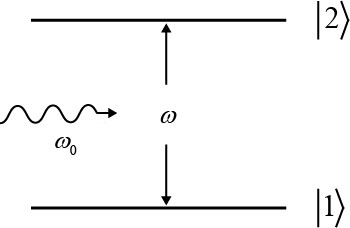
\includegraphics[scale=0.5]{Img/Fig_1.pdf}
	\bicaption{自旋压缩的方案示意图。 激光束进入光学腔并与$x$偏振的集体自旋相互作用以实现基态$\ket{1}$和激发态$\ket{3}$之间的非共振耦合。基态$\ket{2}$通过最初处于真空态的腔模式耦合到激发态$\ket{3}$。绝热消除激发态导致集体自旋的非线性OAT演化。沿着$x$方向向集体旋转并添加均匀磁场B使得能够将OAT转换为TAT自旋压缩。}	
	{Schematic setup for spin squeezing. A laser beam enters the optical cavity and interacts with an $x$-polarized collective spin to realize the off-resonance coupling between the ground state $|1\rangle$ and the exited state $|3\rangle$. The ground state $|2\rangle$ is coupled to the excited state $|3\rangle$ by a cavity mode which is initially in a vacuum state. Adiabatic elimination of the exited state leads to a nonlinear OAT evolution for the collective spin. Adding a homogeneous magnetic field $B$ to the collective spin along the $x$ direction enables the conversion of OAT into TAT spin squeezing.}
	\label{figure7}
\end{figure}
原子被一个频率为$\omega$,拉比频率为$\Omega$的强经典场驱动,驱动场作用在$\ket{1}$和$\ket{3}$的原子跃迁上(其能级差对应的频率为$\omega_{13}$)。腔中的量子场$c$作用在$\ket{2}$和$\ket{3}$的原子跃迁上(其能级差对应的频率为$\omega_{23}$),量子场的频率为$\omega_0$。腔模最初处于真空态,原子最初是处在它们基态的叠加态上,形成自旋相干态(coherent spin state, CSS)$\ket{CSS}=2^{N/2}(\ket{1}+\ket 2)^{\otimes N}$,算符$\hat{S}_x$的本征态的本征值为N/2。经典场从$\ket 1\to\ket 3$谐振的失谐量是$\Delta$[其能极差为$\omega_{13}$(下文中我们取$\hbar=1$)],而量子场与非共振原子跃迁$\ket 1\to\ket 3$(其能极差为 ${\omega _{23}} \equiv {\omega _{13}}$)的失谐量是$\Delta+\delta$,其中$\delta=\omega-\omega_0$是双光子失谐[见图\ref{figure7}]。取基态$\ket{1}$为零势能点,则描述系统的哈密顿量可以写为
\begin{align}
\hat H = {\omega _0}{\hat c^\dag }c + {\sum _k}{\omega _{13}}\ket{3}_k\bra{3}+ {\sum _k}\left( {\frac{\Omega }{2}{e^{ - i\omega t}}\ket{3}_k\bra{1} + g\hat c\ket{3}_k\bra{2} + h.c.} \right),\label{eq441}
\end{align}
其中前两项分别描述腔场和原子的能量,最后一项描述光与原子之间的相互作用,其耦合强度$g=d\sqrt{\omega_0/2\pi\epsilon_0V_0}$,其中$d$是$\ket 2\to\ket 3$的偶极矩,$\epsilon_0$是真空介电常数,$V_0$是模的体积。定义$\hat{\sigma}_{\mu\nu}=\sum_k\ket{\mu}_k\bra{\nu}(\mu,\nu\in{1,2,3})$ ,则体系的哈密顿量可简化为
\begin{align}
\hat H = {\omega _0}{\hat c^\dag }c + {\omega _{13}}{\hat \sigma _{33}} + \frac{\Omega }{2}{e^{ - i\omega t}}{\hat \sigma _{31}} + g\hat c{\hat \sigma _{32}} + \frac{{{\Omega ^*}}}{2}{e^{i\omega t}}{\hat \sigma _{13}} + {g^*}{\hat \sigma _{23}}{\hat c^\dag },\label{eq442}
\end{align}
在$\hat H_0= \omega_0\hat c^\dag \hat c + \omega_{ae}\sigma_{ee}+ \omega_{ab}\sigma_{bb}$的旋转框架下,对公式(\ref{eq442})的哈密顿量进行旋转,得到
\begin{align}\label{eq443}
\begin{split}
\tilde{ \hat{ H}} &= {e^{i{{\hat H}_0}t/\hbar }}\hat H{e^{ - i{{\hat H}_0}t/\hbar }} - {{\hat H}_0}\\
&= \Delta {{\hat \sigma }_{33}} + \frac{\Omega }{2}{{\hat \sigma }_{31}} + g\hat \varepsilon {{\hat \sigma }_{32}} + \frac{{{\Omega ^*}}}{2}{{\hat \sigma }_{13}} + g{{\hat \sigma }_{23}}{{\hat \varepsilon }^\dag },
\end{split}
\end{align}
式中我们定义了一个新算符$\hat \varepsilon  = \hat c{e^{i\delta t}}$。根据哈密顿量,我们可以计算出光和原子的海森堡方程,得到如下的Maxwell-Bloch方程
\begin{align}
{\dot {\hat {\sigma}} _{11}}& = i\frac{\Omega }{2}{\hat \sigma _{31}} - i\frac{{{\Omega ^*}}}{2}{\hat \sigma _{13}},\label{eq444}\\
{\dot {\hat {\sigma}} _{22}} &= ig\hat \varepsilon {\hat \sigma _{32}} - i{g^*}{\hat \sigma _{23}}{\hat \varepsilon ^\dag },\label{eq445}\\
{\dot {\hat {\sigma}} _{12}}& = i\frac{\Omega }{2}{\hat \sigma _{32}} - i{g^*}{\hat \sigma _{13}}{\hat \varepsilon ^\dag },\label{eq446}\\
{\dot {\hat {\sigma}} _{13}} &=  - i\Delta {\hat \sigma _{13}} - i\frac{\Omega }{2}\left( {{{\hat \sigma }_{11}} - {{\hat \sigma }_{33}}} \right) - ig\hat \varepsilon {\hat \sigma _{12}},\label{eq447}\\
{\dot {\hat {\sigma}} _{23}}& =  - i\Delta {\hat \sigma _{23}} - i\frac{\Omega }{2}{\hat \sigma _{21}} - ig\hat \varepsilon \left( {{{\hat \sigma }_{22}} - {{\hat \sigma }_{33}}} \right),\label{eq448}\\
{\dot {\hat {\sigma}} _{33}} &= i\frac{{{\Omega ^{\rm{*}}}}}{2}{\hat \sigma _{13}} - i\frac{\Omega }{2}{\hat \sigma _{31}} + i{g^{\rm{*}}}{\hat \sigma _{23}}{\hat \varepsilon ^ + } - ig\hat \varepsilon {\hat \sigma _{32}},\label{eq449}\\
\dot{ \hat{ \varepsilon}}  &=  - i{g^*}{\hat \sigma _{23}} + i\delta \hat \varepsilon ,\label{eq4410}
\end{align}
接下来,为了方便计算,我们做如下的假设:1.假设经典驱动场足够的弱。2.假设失谐量$\Delta\gg 1$。通过这样的假设,可以认为布居在激发态的原子数非常少,因此可以绝热消除掉激发态(${\hat{\sigma} _{33}} \simeq 0$)。大失谐还可以将$\hat{\sigma}_{13}$和$\hat{\sigma}_{23}$快速驱动到稳态,于是有${\hat \sigma _{13}} \simeq  - \left( {\Omega {{\hat \sigma }_{11}}/2 + g\hat \varepsilon {{\hat \sigma }_{12}}} \right)/\Delta $,${\hat \sigma _{23}} \simeq  - \left( {\Omega {{\hat \sigma }_{21}}/2 + g\hat \varepsilon {{\hat \sigma }_{22}}} \right)/\Delta $ 。我们进一步假设双光子失谐量足够大$\delta\gg 1$,使得在相互作用期间腔中没有产生显着的光子激发,这使得能够绝热地消除腔场,导致$\hat \varepsilon  =  - {g^*}\Omega {\hat \sigma _{21}}/2\Delta \delta $。基于这些假设,原子的基态方程可以写为
\begin{align}
{\dot{ \hat{ \sigma }}_{12}} =  - i{\kappa _0}{\hat S_z}{\hat \sigma _{12}} - i{\chi _0}{\hat \sigma _{12}},{\dot{ \hat{ \sigma }} _{11}} = {\dot{ \hat{ \sigma }} _{22}} = 0,\label{eq4411}
\end{align}
其中定义了 $\kappa_0=|\Omega|^2{|g|^2}/4{\delta\Delta^2}$ 和 $\chi_0 ={|\Omega|^2}/{4\Delta}$,以及角动量算符${\hat S_x} = (\hat{\sigma}_{12}+\hat{\sigma}_{21})/2$,${\hat S_y} = (\hat{\sigma}_{12}-\hat{\sigma}_{21})/2i$和${\hat S_z} = (\hat{\sigma}_{11}-\hat{\sigma}_{22})/2$。在伪角动量运算符的表述中,公式(\ref{eq4411})可以写为
\begin{align}
{{\dot {\hat S}}_x} &= {\kappa _0}\left( {{{\hat S}_y}{{\hat S}_z} + {{\hat S}_z}{{\hat S}_y}} +{{\hat S}_y}\right) + {\chi _0}{{\hat S}_y},\label{eq4412}\\
{{\dot {\hat S}}_y} &=  - {\kappa _0}\left( {{{\hat S}_x}{{\hat S}_z} + {{\hat S}_z}{{\hat S}_x}} +{{\hat S}_x}\right) - {\chi _0}{{\hat S}_x},\label{eq4413}\\
{{\dot {\hat S}}_z} &= 0,\label{eq4414}
\end{align}
从上面的这组方程,可以推断原子的动力学是由下式的有效哈密顿量产生的
\begin{align}
\hat H_{eff}=-\chi_0\hat S_z-\kappa_0(\hat S_z+\hat S_z^2),\label{eq4415}
\end{align}
从哈密顿量的形式我们知道这是一个OAT型的哈密顿量\cite{PRA1993Kitagawa}。(\ref{eq4415})式的第一项出现源于基态的AC-Stark平移,而其余项源于双光子非共振拉曼跃迁。通过考虑如图\ref{figure7}(b)所示的双拉曼过程,可以理解(\ref{eq4415})式中的非线性项的来源。假设所有原子在基态$\ket{1}$从经典驱动场吸收一个光子,并向腔场辐射一个光子,该光子被基态$\ket{2}$中的另一个原子吸收, 然后再次回到经典驱动场,这将导致从$\ket{12}\to\ket{21}$的有效转换。这双原子过程保持共振并导致自旋-自旋纠缠(以及自旋压缩)的产生。这种双原子翻转的动力学可以用有效的哈密顿量${\hat H_{eff}} = {\hat S_ - }{\hat S_ + } \propto \hat S_z^2$来描述。应该提到的是,原子发射的腔光子有可能被原子本身吸收,这抑制双原子过程。这就是为什么我们在这里采用相等的叠加自旋态作为输入态,因为在这种态下参与腔-光子反复吸收的原子数约为N/2,这可以极大地抑制自重吸收的影响,因此使双原子过程占主导地位。

我们可以很容易的求解方程(\ref{eq4412})得到
\begin{align}\label{eq4416}
\begin{split}
{{\hat S}_x}(t) =& {{\hat S}_ + }(0)\exp [i\mu ({{\hat S}_z} + 1/2 + \varphi /\mu )] \\
&+ \exp [ - i\mu ({{\hat S}_z} + 1/2 + \varphi /\mu )]{{\hat S}_ + }(0),
\end{split}
\end{align}
其中$\mu = -2\kappa_0 t$,$\varphi = -\varphi_0 t$和$\varphi_0=\chi_0+\kappa_0$。
将CSS在Dicke态的基上展开
\begin{align}
\ket{CSS} = \sum\nolimits_{m=-S}^S 2^{ - S}\sqrt {(2S)!/[(S + m)!(S - m)!]}\ket{m},\label{eq4417}
\end{align}
$S_x$的平均值通过计算可得
\begin{align}
\bra{CSS}\hat {S}_x\ket{CSS}=S \cos^{2S-1}{\frac {\mu}2} \cos{ \varphi },\label{eq4418}
\end{align}
对于$S\gg 1$和 $|\mu|,|\varphi|\ll1 $,有$\braket{S_x}\simeq S$。
这意味着在OAT相互作用之后,几乎所有原子仍然沿$x$方向极化。因此可以使用Holstein-Primakoff近似\cite{PhysRevA.58.1098}来定义新的原子量子变量$\hat {X}_a = {\hat S_y}/\sqrt {S_x} ,{\hat P_a} = {\hat S_z}/\sqrt {S_x} $,
满足$[\hat {X}_a,\hat {P}_a] = i$,对于CSS,有$\braket{\hat {X}_a}=\braket{\hat {P}_a}=0$
和归一化方差$(\Delta {\hat X}_a)^2 =(\Delta {\hat P}_a)^2= 1/2$。对于这种定义,方程(\ref{eq4413}-\ref{eq4414})可以表述为
\begin{align}
\hat X_a^{out} = \hat X_a^{in} + \alpha \hat P_a^{in} + \beta ,\hat P_a^{out} = \hat P_a^{in},\label{eq4419}
\end{align}
其中“in”和“out”是指相互作用之前和之后的原子,我们定义了耦合常数$\alpha=S\mu$和由于哈密顿量(\ref{eq4415})式中的线性项引起的位移参数$\beta=\sqrt{S}\phi$。显然,(\ref{eq4419})式中的自旋态是通过$\hat{P}_a^2$中哈密顿量的二次项来进行第一次压缩的自旋态,然后通过移位量$\beta$在相空间沿着$\hat{P}_a$方向来取代自旋压缩态而产生的。由于相空间中的位移运算(线性运算)不会减少由OAT演化\cite{RevModPhys.77.513}产生的原子-原子纠缠,因此当我们估计原子系统的压缩量时,可以忽略位移$\beta$。为了看看产生了多少压缩,我们通过幺正变换$\hat X_\theta^{out}=\exp(i\theta\hat H_{SR}) \hat X_a^{out}\exp(-i\theta\hat H_{SR})=\cos{\theta} \hat X_a^{in}+(\alpha\cos{\theta}+\sin{\theta})\hat P_a^{in}$绕$x$轴旋转自旋态,其中 $\hat H_{SR}=-2\hat S_x\simeq \hat X_a^2+\hat P_a^2$是自旋旋转哈密顿量\cite{PhysRevLett.91.060401}。关于$\theta$我们求方差$(\Delta\hat X_\theta^{out})^2$的最佳值,我们得到$\xi_{OAT}^2=2(\Delta\hat X_\theta^{out})^2=1+\alpha^2/2-(\alpha^4/4+\alpha^2)^{1/2}\Rightarrow \mathop{\lim}\limits_{\alpha\rightarrow \infty}1/\alpha^2$,其中$\theta=\arctan (2/\alpha)/2+\pi/2$。

如果可以将OAT转化为TAT,那么压缩量可以大大增加\cite{PhysRevLett.107.013601}。为此,我们在OAT相互作用过程中添加一个围绕$x$方向的旋转角频率$\Omega_0$ \cite{PhysRevA.92.063610,PhysRevA.87.051801,PhysRevA.91.053826}(可以通过沿$x$轴施加均匀磁场来实现,如图\ref{figure7}所示),于是将得到哈密顿量
\begin{align}\label{eq4420}
\begin{split}
\hat H_{TAT}&=\Omega_0\hat H_{SR}/2+\hat H_{eff}\\
            &=\Omega_0(\hat X_a^2+\hat P_a^2)/2-\kappa_0 S\hat P_a^2\\
            &=\kappa_0S(\hat X_a^2-\hat P_a^2)/2,
\end{split}
\end{align}
其中$\Omega_0=\kappa_0S$,这正是TAT型相互作用\cite{PRA1993Kitagawa},并以一个与耦合常数呈指数级缩放的速率压缩自旋涨落,即$\xi^2_{TAT}=\exp(-\alpha)$。与产生多项式压缩的OAT相比,TAT方法的指数缩放将极大地增强各个原子之间的纠缠,从而使我们能够对集体自旋进行很重要的控制。

\vbox{}
\section{噪声对方案的影响}
\vbox{}
到目前为止,我们忽略了噪声的影响。实际上,光子以一定的速率$\kappa$从空腔泄漏到环境中,激发态以辐射衰减率$\gamma_{13}=\gamma_{23}\equiv \gamma$衰减到基态。在存在衰变以及绕$x$方向旋转的情况下,原子算符的时间演变(更多详细推导参见附录\ref{appendix})可写为
\begin{eqnarray}
\frac{d}{{dt}}\left( {\begin{array}{*{20}{l}}
	{{{\hat X}_a}}\\
	{{{\hat P}_a}}
	\end{array}} \right) = \mathcal{G}\left( {\begin{array}{*{20}{l}}
	{{{\hat X}_a}}\\
	{{{\hat P}_a}}
	\end{array}} \right) - \sqrt S \left( {\begin{array}{*{20}{l}}
	{\varphi_0}\\
	\eta
	\end{array}} \right)
+ \sqrt {2\eta } \left( {\begin{array}{*{20}{l}}
	{{{\hat {\mathcal{F}}}_y}}\\
	{{{\hat {\mathcal{F}}}_z}}
	\end{array}} \right)\label{eq4421}
\end{eqnarray}
对于$r_0=\kappa/2\delta\ll 1$的情况
\begin{eqnarray}
\mathcal{G}={\Omega _0}\left( {\begin{array}{*{20}{c}}
	0&{ 1}\\
	-1&0
	\end{array}} \right) - 2S{\kappa _0}\left( {\begin{array}{*{20}{c}}
	0&1\\
	0&0
	\end{array}} \right) - \eta \left( {\begin{array}{*{20}{c}}
	1&0\\
	0&1
	\end{array}} \right),\label{eq4422}
\end{eqnarray}
在上式中$\eta=\chi_0\gamma/\Delta$表示原子的衰减参数,$\hat {\mathcal{F}}_y$和$\hat {\mathcal{F}}_z$是朗之万噪声算符,满足$\braket{\hat{\mathcal{F}}_y(t) \hat{\mathcal{F}}_z(t')}= i\delta(t-t')/2$和 $
\braket{\hat{\mathcal{F}}_y(t)\hat{\mathcal{F}}_y(t')}=\braket{\hat{\mathcal{F}}_z(t)\hat{\mathcal{F}}_z(t')}=\delta(t-t')/2$。$\mathcal{G}$的第一项表示原子由于$\Omega_0$绕$x$轴转动,$\mathcal{G}$中的第二项表示由光引起的相干OAT相互作用,而第三项表示由光泵浦引起的原子的横向衰变。注意,$\hat{P}_a$现在也以与$\eta$成比例的速率变化,这是由于强光场的作用导致基态布居数从$\ket{1}$转移到$\ket{2}$引起的。这个微分方程的解是
\begin{eqnarray}
\left( {\begin{array}{*{20}{l}}
	{\hat X_a^{out}}\\
	{\hat P_a^{out}}
	\end{array}} \right) &=& \mathcal{A}\left( t \right)\left( {\begin{array}{*{20}{l}}
	{\hat X_a^{in}}\\
	{\hat P_a^{in}}
	\end{array}} \right) - \mathcal{A}\left( t \right)\int_0^t {d\tau {\mathcal{A}^{ - 1}}\left( \tau  \right)} \nonumber\\
&&\times \left[ {\sqrt S \left( {\begin{array}{*{20}{l}}
		{{\varphi _0}}\\
		\eta
		\end{array}} \right) - \sqrt {2\eta } \left( {\begin{array}{*{20}{l}}
		{{{\hat {\mathcal{F}}}_y\left( \tau \right)}}\\
		{{{\hat {\mathcal{F}}}_z\left( \tau \right)}}
		\end{array}} \right)} \right],\label{eq4423}
\end{eqnarray}
其中齐次解为$\mathcal{A}\left( t \right)=\exp(\mathcal{G}t)$。对于OAT压缩的情况($\Omega_0=0$),我们有%$\mathcal{A}(t)={e^{ - \eta t}}\bigl(\begin{smallmatrix} 1 & \alpha \\\alpha & 0 \end{smallmatrix}\bigr)$
$$\mathcal{A}(t)={e^{ - \eta t}}\left(\begin{array}{cc}
1 & \alpha \\
\alpha & 0
\end{array}\right)$$
我们也可以直接从公式(\ref{eq4423})得到
\begin{eqnarray}
\hat X_a^{out} &=& \sqrt {1 - {\eta _0}} \left( {\hat X_a^{in} + \alpha \hat P_a^{in} + \beta' } \right) + \sqrt {{\eta _0}} {{\hat{\mathcal{F}}}_X},\label{eq4424}\\
\hat P_a^{out} &=& \sqrt {1 - {\eta _0}} \left( {\hat P_a^{in} + \beta ''} \right) + \sqrt {{\eta _0}} {{\hat{{\mathcal{F}}}}_P},\label{eq4425}
\end{eqnarray}
其中我们定义了参数$\eta_0=2\eta t, \beta'=\beta+\eta_0\alpha/4$和 $\beta''=\sqrt{S}\eta_0/2$,并使用了条件 $\eta_0\ll 1$。修改后的噪声算子的形式如下:$\hat{\mathcal{F}}_X=\frac{1}{\sqrt t}e^{-\eta t}\int_0^td\tau e^{\eta \tau}[\hat{\mathcal{F}}_y(\tau)-\alpha(\tau-t)/t\hat{\mathcal{F}}_z(\tau)],\hat{\mathcal{F}}_P=\frac{1}{\sqrt t}e^{-\eta t}\int_0^td\tau e^{\eta \tau}\hat{\mathcal{F}}_z(\tau)$, 我们也可以很容易的得到$\langle\hat{\mathcal{F}}_X\rangle=\langle \hat{\mathcal{F}}_P\rangle=0,\langle\hat{\mathcal{F}}_X \hat{\mathcal{F}}_P\rangle\simeq i(1-i\alpha/2)/2$,$\langle\hat{\mathcal{F}}_X^2\rangle\simeq (1+\alpha^2/3)/2$和 $\langle \hat{\mathcal{F}}_P^2\rangle\simeq 1/2$。借助于原子输入-输出关系(\ref{eq4424})和(\ref{eq4425}),我们可以计算方差$(\Delta\hat X_\theta^{out})^2$,从而得到方差的最优值
\begin{align}\label{eq4426}
\begin{split}
2(\Delta\hat X_\theta^{out})^2 =& 1 + \frac{{{\alpha ^2}}}{2}\left( {1 - \frac{2}{3}{\eta _0}} \right)\\
&- \sqrt {{{\left( {1 - \frac{2}{3}{\eta _0}} \right)}}^2\frac{{{\alpha ^4}}}{4} + {{\left( {1 - \frac{1}{2}{\eta _0}} \right)}}^2{\alpha ^2}}\\
&\Rightarrow \frac{1}{\alpha^2}+\frac{\eta_0}{3},\qquad\qquad\alpha \gg 1,
\end{split}
\end{align}
其中$\theta=\arctan [(2-\eta_0)/(\alpha-2\eta_0\alpha/3)]/2+\pi/2$。方程(\ref{eq4426})表明原子衰减设有一个极限,即$\eta_0/3$,达到了可以达到的最高压缩程度。对于位于腔体波腹上的原子,耦合常数$g$还可以方便地用激发态线宽$|g|^2=\gamma\kappa d_c/(4N)$表示\cite{phd11},腔体光学深度(optical depth, OD)为$d_c=\frac{2\mathcal {F}}{\pi}d_0=\frac{2\mathcal {F}}{\pi}\frac{N\sigma_0}{A_0}$,其中$\mathcal {F}$是腔体精细度,$d_0=N\sigma_0/A_0$是自由空间样品的OD值,$\sigma_0$是原子的光子吸收截面,$A_0$是波腹的有效截面积。然后可以将耦合常数$\alpha$重新表达为$\alpha=r_0 d_c\eta_0/2$。因此,对于大$\alpha$的压缩量可以写为$2(\Delta\hat X_\theta^{out})^2= 1/(r_0 d_c\eta_0/2)^2+\eta_0/3\geq 3^{1/3}/(r_0 d_c)^{2/3}\propto 1/N^{2/3}$,这正是如上所述的OAT缩放。

对于TAT的压缩($\Omega_0=S\kappa_0$),我们有$$\mathcal{A}(t)=e^{-\eta t}\left( {\begin{array}{*{20}{c}}
	\cosh\frac{\alpha}{2}&-\sinh\frac{\alpha}{2} \\
	-\sinh\frac{\alpha}{2}&\cosh\frac{\alpha}{2}
	\end{array}} \right)$$因此可以从方程(\ref{eq4426})推导出原子正交$\hat X_{\pi/4}$的输入-输出关系
\begin{eqnarray}
\hat X_{\frac{\pi }{4}}^{out}{\rm{ }} = \sqrt {1 - {\eta _0}} \left[ {{e^{ - \frac{\alpha }{2}}}\hat X_{\frac{\pi }{4}}^{in} + \frac{{ {\beta  - \beta ''} }}{{\sqrt 2 }}} \right] + \sqrt {{\eta _0}} {\hat {\mathcal{F}}_{\frac{\pi }{4}}},\label{eq4427}
\end{eqnarray}
其中 ${\hat {\mathcal{F}}_{\frac{\pi }{4}}}=\frac{1}{\sqrt{2t}}e^{-(\eta_0+\alpha)/2}\int^t_0d\tau e^{(\eta+S\kappa_0)\tau}[{\hat {\mathcal{F}}_{z}}(\tau)-{\hat {\mathcal{F}}_{y}}(\tau)]$。它的方差可以直接计算得出
\begin{align}\label{eq4428}
\begin{split}
2(\Delta\hat X_{\frac{\pi }{4}}^{out})^2=
&\left(1-\eta_0\right)e^{-\alpha}+\frac{\eta_0\left[1-(1-\eta_0)e^{-\alpha}\right]}{\eta_0+\alpha}\\
&\Rightarrow \frac{\eta_0}{\alpha}\propto\frac{1}{N},\qquad\qquad\alpha\gg 1,
\end{split}
\end{align}
这表示TAT方案可以是压缩达到海森堡极限。此外,还需要根据方程(\ref{eq443})中给出的定义考虑$x$分量衰减的影响,即${\langle {\hat S_x}\rangle ^2} \simeq (1 - {\eta _0})N/2$  [可以从式(\ref{a2})推导得出]。

\begin{figure}[htbp]
	\centering
	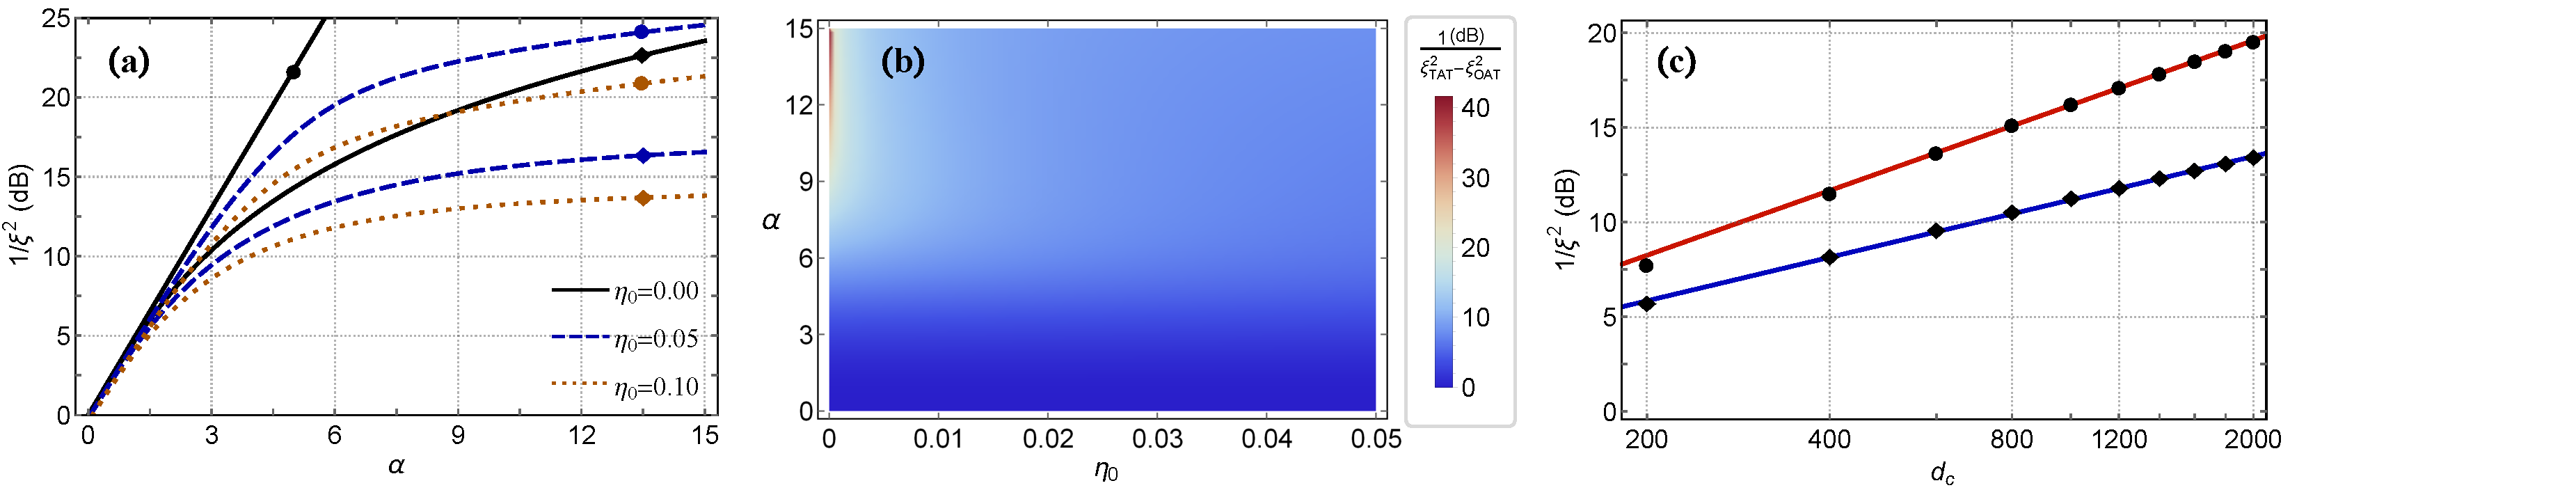
\includegraphics[scale=0.26]{Img/Fig_2.pdf}
	\bicaption{
		(a)OAT(带有菱形的线)和TAT(带圆圈的线)协议的性能随着各种原子衰变值的耦合强度$ \alpha $而变化的曲线。
		(b)两个方案产生的压缩度之差随耦合强度$ \alpha $和原子衰变$ \eta_0 $的变化。 
		(c)为$r_0 = 0.1$时OAT(钻石线)和TAT(圆圈线)方案随腔OD $d_c$变化的最佳挤压效果。}
	{
		(a) Performance of OAT (lines with diamond) and TAT (lines with circle) protocols varies with coupling strength $\alpha$ for various values of atomic decay. 
		(b) Squeezing difference of the two proposed squeezing protocols versus coupling strength $\alpha$ and atomic decay $\eta_0$. 
		(c) Best achievable squeezing of OAT (line with diamonds) and TAT (line with circles) protocols versus cavity OD dc for $r_0=0.1$.}
		\label{figure42}
\end{figure}

  我们首先计算了压缩参数$\xi^2\simeq2(\Delta\hat{X}_\theta^{out})^2/(1-\eta_0)$并绘制图\ref{figure42},在图(a)中我们绘制了依赖于耦合强度$\alpha$的各种原子衰变值的压缩量。从中可以看出如果原子衰变小于10\%,那么对于相互作用参数$\alpha=5$,可以获得大于10dB的压缩度。此外,正如预期的那样,TAT协议比OAT协议更加有效,即使在有噪音的情况下。对协议性能与原子衰减的进一步研究(如图(b)所示)表明TAT协议对于噪声更加敏感,相反,OAT协议对原子衰变显得更加稳定。因此,对于TAT协议,我们需要极低的衰减率来保留它的优点。在实际实现中,使用可访问的实验参数OD来评估所提议的协议的性能是非常方便的。在图(c)中,我们绘制了两个所提协议相对于腔OD$d_c$的最佳可实现的压缩图像(相对于$\eta_0$优化)。对于自由空间OD大约为30\cite{JPB2008qf}的室温蒸汽,如果设置参数$r_0=0.1$和精细$F\simeq100$,OAT和TAT产生的压缩度将分别达到13.4dB和19.6dB。

  我们对于具体的实验实现也进行了相关的参数估计。我们考虑一个含有$5\times 10^6$个原子的原子样品,并选择一个真实的腔耦合参数$g=(2\pi)100kHz$。如果选择参数$\gamma=\kappa\sim10^2g$,$\Omega\sim10^4g$,$\Delta\sim10^5g$和$\delta\sim5\times10^2g$,取$\alpha\simeq5$,我们将得到相互作用时间$t$大约在$0.3\mu s$左右,在$\eta_0<10\%$,$r_0\ge1$的情况下,最终我们将得到大于10dB的压缩度。
  
\vbox{}
\section{结论}
\vbox{}
  我们提出了一种在光学腔中原子系综产生高度自旋压缩态的方案。该过程基于光和自旋极化原子系综之间的非共振SRS相互作用。通过向放置在最初处于真空态的光学腔中的极化原子蒸汽发送强脉冲,我们发现可以实现OAT压缩。腔场与原子之间的相互作用越强,压缩程度越高。我们还表明,通过沿自旋极化方向添加均匀磁场,可以将OAT协议转换为更有效的TAT协议。我们在不同噪声的影响下对方案进行测试,我们发现如下的特点:

    (1)即使在存在大约10\%的原子发生衰减的情况下,我们的体系仍然可以获得大于10dB的压缩;

    (2)尽管TAT协议的性能一般来说要比OAT协议更有优异,但是其对于原子的衰减却更加敏感;

    (3)OAT协议在对抗噪声的影响方面显得叫TAT协议更加强大。

  因此,我们认为尽管OAT协议在压缩方面并不优于TAT协议,但它在嘈杂的环境中易于存活的良好特性以及更简单的实验设置使其适用于各种原子系统。我们期望所提出的协议在量子信息处理和量子计量的背景下是有益的。



